%====================================================
\section{Linear Advection With Constant Coefficients}\label{chap:advection}
%====================================================


\begin{figure}[htbp]
	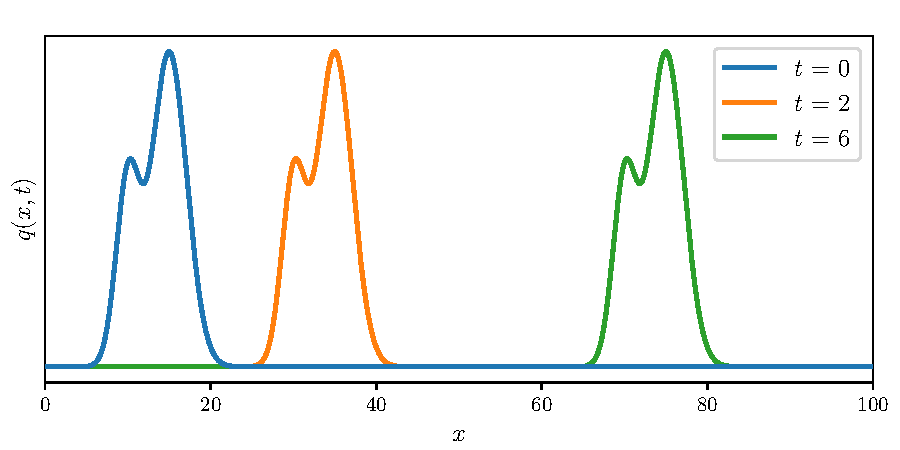
\includegraphics[width=\textwidth]{figures/linear_advection_solution.pdf}%
	\caption{
		The analytical solution of the linear advection equation with constant
		coefficients (eq. \ref{eq:advection-equation}). The solution consists
		of the same initial shape being translated with $a t$ as time evolves.
	}
	\label{fig:advection-analytical-solution}
\end{figure}


In principle, we're trying to solve a class of partial differential equations called
``Hyperbolic Conservation Laws''. They are determined by a ``state vector'' $\U$ and
a ``flux tensor'' $\F(\U)$ (in addition to a couple of other conditions on the relation between
$\U$ and $\F(\U)$ which don't really matter for this exercise.) Hyperbolic conservation
laws take the following form:

\begin{equation}
	\DELDT{ \U } + \nabla \cdot \F (\U) = 0
\end{equation}

In this exercise, we're focussing on the so-called ``linear advection with constant
coefficients'', which is given by

\begin{align}
	\U(\x, t) &= q(\x, t) \\
	\F(\U(\x, t)) &= a \cdot q(\x, t) \quad , \quad a = \text{ const } > 0
\end{align}

effectively giving us in 1D:

\begin{equation}
\boxed{
	\DELDT{ q } + a \cdot \DELDX{q} = 0 \label{eq:advection-equation}
}
\end{equation}

The analytical solution is given by any function $q(x)$ which satisfies

\begin{equation}
	q(x, t) = q(x - a (t - t_0), t_0) \label{eq:advection-solution}
\end{equation}

This can readily be verified by applying the time derivative (and the following
chain rule) to the function \ref{eq:advection-solution}

\begin{align}
	\deldt q(x, t) = \deldt q(x - a(t - t_0), t_0)
		= \deldx{q(x, t_0)} \cdot  \deldt{\left( - a(t - t_0) \right)}
		= - a \deldx{q(x, t_0)} \label{eq:advection-derivative}
\end{align}

Inserting \ref{eq:advection-derivative} into \ref{eq:advection-equation}
instantly shows that the original equation \ref{eq:advection-equation} is satisfied.

The solution \ref{eq:advection-solution} describes a function $q(x, t)$ of any
arbitrary shape being translated by $a t$ as time evolves. See
Figure~\ref{fig:advection-analytical-solution} for a visualization.


